%% Standalone figure source (JIIS submission). Generated from the KBS
%% version, content unchanged unless wrapped in ... (red).
\documentclass[border=0pt]{standalone}
% =====================================================================
% Shared preamble of the standalone figure sources (Fig3, Fig4, Fig5,
% Fig6, Fig7). Each figure is compiled on its own to FigN.pdf, because
% the JIIS guidelines ask for figures supplied as separate files named
% "Fig" + number, uploaded without subfolders.
%
% Every figure body sits in a 119mm minipage: the JIIS figure width for
% small-format journals (single-column body), and main.tex includes each
% PDF at its natural size.
% =====================================================================
\usepackage[utf8]{inputenc}
\usepackage[T1]{fontenc}
\usepackage{amsmath,amssymb,amsfonts}
\usepackage{textcomp}
\usepackage{xcolor}
\usepackage{tikz}
\usetikzlibrary{arrows.meta, positioning, calc, fit, backgrounds}
\usepackage{pgfplots}
\pgfplotsset{compat=1.18}

% --- figure palette (matches the repository architecture diagram) ---
\definecolor{figamber}{HTML}{F59E0B}
\definecolor{figcyan}{HTML}{06B6D4}
\definecolor{figsky}{HTML}{0EA5E9}
\definecolor{figviolet}{HTML}{8B5CF6}
\definecolor{figgold}{HTML}{EAB308}
\definecolor{figgreen}{HTML}{10B981}
\definecolor{figpink}{HTML}{EC4899}
\definecolor{figred}{HTML}{DC2626}

% --- OPENER-ZS operating points ---
\newcommand{\zstr}{OPENER-ZS\textsubscript{trans}}
\newcommand{\zsind}{OPENER-ZS\textsubscript{ind}}

\begin{document}
\begin{minipage}{160mm}
\centering
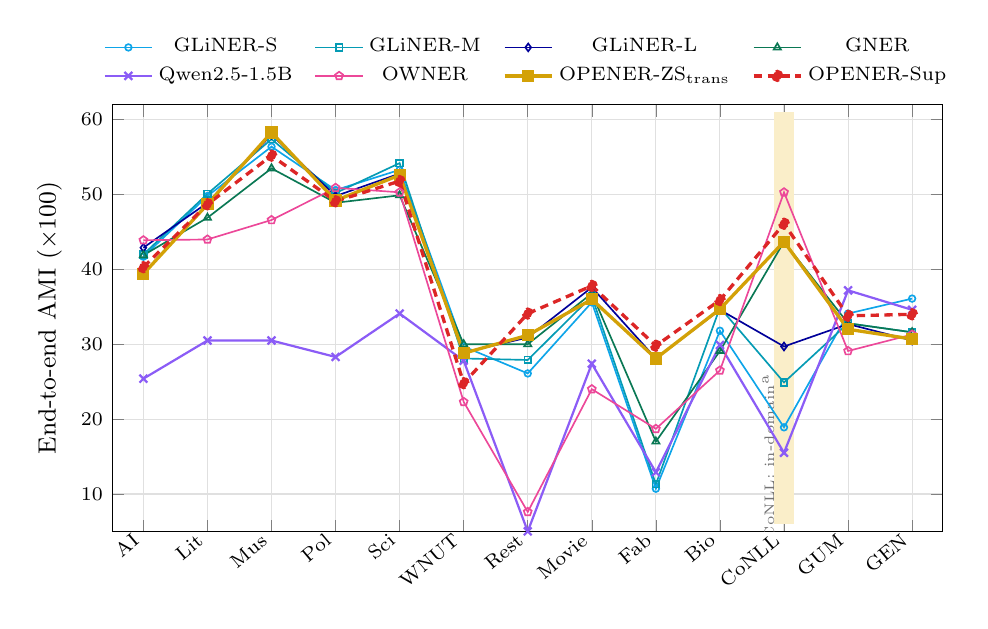
\begin{tikzpicture}
\begin{axis}[
  width=\linewidth, height=7.0cm,
  ymin=5, ymax=62,
  ylabel={End-to-end AMI ($\times100$)}, ylabel style={font=\small},
  symbolic x coords={AI,Lit,Mus,Pol,Sci,WNUT,Rest,Movie,Fab,Bio,CoNLL,GUM,GEN},
  xtick=data, xticklabel style={rotate=40, anchor=east, font=\scriptsize},
  ytick={10,20,30,40,50,60}, yticklabel style={font=\scriptsize},
  grid=both, major grid style={black!12},
  enlarge x limits=0.04,
  legend style={at={(0.5,1.02)}, anchor=south, legend columns=4, font=\scriptsize, draw=none,
                /tikz/every even column/.append style={column sep=6pt}},
]
% in-domain CoNLL band (drawn first -> behind the curves)
\draw[figgold!22, line width=7pt] (axis cs:CoNLL,6) -- (axis cs:CoNLL,61);
\node[font=\tiny, black!55, rotate=90, anchor=south] at (axis cs:CoNLL,15) {CoNLL: in-domain\textsuperscript{a}};
%       --       zero-shot systems (solid)       --
\addplot[figsky, semithick, mark=o, mark size=1.2pt] coordinates
  {(AI,41.7)(Lit,49.8)(Mus,56.4)(Pol,50.6)(Sci,53.3)(WNUT,29.7)(Rest,26.1)(Movie,35.6)(Fab,10.7)(Bio,31.8)(CoNLL,18.9)(GUM,34.1)(GEN,36.1)};
\addplot[figcyan!85!black, semithick, mark=square, mark size=1.2pt] coordinates
  {(AI,42.0)(Lit,50.1)(Mus,57.4)(Pol,50.2)(Sci,54.2)(WNUT,28.1)(Rest,27.9)(Movie,36.4)(Fab,11.3)(Bio,34.9)(CoNLL,24.9)(GUM,32.8)(GEN,31.6)};
\addplot[blue!60!black, semithick, mark=diamond, mark size=1.4pt] coordinates
  {(AI,42.9)(Lit,48.9)(Mus,58.0)(Pol,49.8)(Sci,52.8)(WNUT,28.9)(Rest,30.9)(Movie,37.6)(Fab,28.1)(Bio,34.6)(CoNLL,29.7)(GUM,32.7)(GEN,30.5)};
\addplot[figgreen!65!black, semithick, mark=triangle, mark size=1.5pt] coordinates
  {(AI,41.9)(Lit,46.9)(Mus,53.5)(Pol,48.9)(Sci,49.9)(WNUT,30.0)(Rest,30.0)(Movie,36.8)(Fab,17.0)(Bio,29.1)(CoNLL,43.7)(GUM,32.8)(GEN,31.6)};
% Qwen2.5-1.5B (4-bit) -- small LLM baseline, zero-shot prompting (150-sentence subsample)
\addplot[figviolet, thick, mark=x, mark size=2pt] coordinates
  {(AI,25.4)(Lit,30.5)(Mus,30.5)(Pol,28.3)(Sci,34.1)(WNUT,27.8)(Rest,5.0)(Movie,27.4)(Fab,12.9)(Bio,29.9)(CoNLL,15.5)(GUM,37.2)(GEN,34.6)};
\addplot[figpink, semithick, mark=pentagon, mark size=1.5pt] coordinates
  {(AI,43.9)(Lit,44.0)(Mus,46.6)(Pol,50.9)(Sci,50.3)(WNUT,22.3)(Rest,7.6)(Movie,24.0)(Fab,18.7)(Bio,26.5)(CoNLL,50.3)(GUM,29.1)(GEN,31.3)};
\addplot[figgold!90!black, very thick, mark=square*, mark size=1.6pt] coordinates
  {(AI,39.4)(Lit,48.7)(Mus,58.3)(Pol,49.2)(Sci,52.6)(WNUT,28.8)(Rest,31.2)(Movie,36.0)(Fab,28.1)(Bio,34.7)(CoNLL,43.7)(GUM,32.0)(GEN,30.7)};
%       --       supervised (dashed)       --
\addplot[figred, very thick, densely dashed, mark=*, mark size=1.6pt] coordinates
  {(AI,40.3)(Lit,48.7)(Mus,55.2)(Pol,49.1)(Sci,51.8)(WNUT,24.8)(Rest,34.1)(Movie,37.8)(Fab,29.8)(Bio,35.9)(CoNLL,46.1)(GUM,33.8)(GEN,34.0)};
\legend{GLiNER-S, GLiNER-M, GLiNER-L, GNER, Qwen2.5-1.5B, OWNER, \zstr, OPENER-Sup}
\end{axis}
\end{tikzpicture}
\end{minipage}
\end{document}
